\documentclass{standalone}
\usepackage{tikz}

\begin{document}
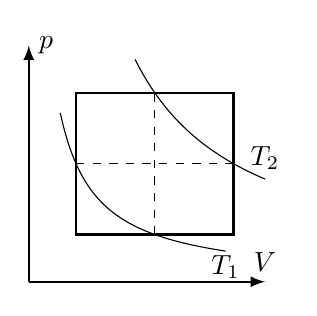
\begin{tikzpicture}
	\draw[thick, arrows={-latex}] (0,0) -- (3,0) node[above] {$V$};
	\draw[thick, arrows={-latex}] (0,0) -- (0,3) node[right] {$p$};
	\draw [thick] (0.6,2.4) rectangle (2.6,0.6);
	\draw plot[dashed, variable=\t, domain=1.35:3, samples=100] ({\t},{4/(\t+0.0666)}) node [above] {$T_2$};
	\draw plot[dashed, variable=\t, domain=0.4:2.5, samples=100] ({\t},{1/(\t+0.0666)}) node [below=-2pt] {$T_1$};
	\draw [dashed] (1.6, 0.6) -- (1.6, 2.4);
	\draw [dashed] (0.6, 1.5) -- (2.6, 1.5);
\end{tikzpicture}
\end{document}